\documentclass{beamer}
\usefonttheme[onlylarge]{structuresmallcapsserif}
\usefonttheme[onlysmall]{structurebold}
\usetheme{Warsaw}
\setbeamercovered{transparent}
%-----------------------------------------Paquetes y comandos personales-------------------------------%
\usepackage{fancybox,color,tcolorbox}
\usepackage{verbatim}
\usepackage[english,spanish,activeacute]{babel}
%\usepackage[latin1]{inputenc}
\usepackage{inputenc}
\usepackage{latexsym}
\usepackage{amsmath}
\usepackage{graphicx} % Allows including images
\usepackage{booktabs}
\usepackage{amssymb}
\usepackage{multimedia}
\usepackage{pifont,pgfcore}
\usepackage{tcolorbox}
\usepackage{animate}
\usepackage{ucs}
\renewcommand\tabularxcolumn[1]{m{#1}}  % for vertical centering of X cell contents
\setlength\tabcolsep{12pt}              % increase horizontal space around cell         \begin{table}
\bfseries
\usepackage{cellspace, tabularx}    % for adding vertical space around cells' contents
\setlength\cellspacetoplimit{7pt}
\setlength\cellspacebottomlimit{7pt}
\newcolumntype{C}{>{\centering\arraybackslash}X}
\addparagraphcolumntypes{C}
\usepackage{ragged2e}
\newcommand\scalemath[2]{\scalebox{#1}{\mbox{\ensuremath{\displaystyle #2}}}}
%-----------------------------------------------------Nuevos Ambientes----------------------------------%

\newtheorem*{Theorem*}{Teorema}
\newtheorem*{Definition*}{Definici\'on}
\newtheorem*{Example*}{Ejemplo}

%-----------------------------------------------------Nuevos Comandos-----------------------------------%
%-----------------------------------------------------Titulo--------------------------------------------%

\vspace*{-0.8cm}
\title[T\'itulo del trabajo]{T\'itulo de la presentaci\'on del trabajo}
\author[Machado, Toledo, Moreno, Concepci\'on, Navarro]
		{
			Daniel Machado \\
			Daniel Toledo \\
			Osvaldo Moreno \\
			Jos\'e A. Concepci\'on \\
			Adri\'an Navarro \\
			{\small C211}
		}
			
\date{Mayo 2023}

\begin{document}
%-----Redefiniendo colores----------%
\definecolor{green}{rgb}{0.1,0.5,0.3}
\definecolor{vio}{rgb}{0.8,0.5,0.2}
\definecolor{g}{rgb}{0.93,0.93,0.93}
\begin{frame}

	\titlepage
	\vspace*{-0.65cm}
	\begin{center}
		\colorbox{black}{\textbf{\begin{large}\textcolor{white}{Defensa del proyecto final.}\end{large}}}\\\ \\
		\vspace*{-0.3cm}
		\scriptsize \textbf{\textcolor{blue}{Facultad Matem\'atica Computaci\'on}}\\
		\textbf{\textcolor{blue}{Universidad de La Habana}}
	\end{center}
\end{frame}
%-----------------------------------------------

%-------------------------------------------------
\begin{frame}
	\frametitle{Temas a tratar}
	\tableofcontents
\end{frame}
%------------------------------------

%-------------------------------------
\section{Introducci\'on}
\begin{frame}
	\begin{minipage}{10cm}
		El artículo titulado "Local Analysis of the Prey-Predator Model with Stage-Structure Prey and Holling
		Type Functional Responses" por Dian Savitri analiza el modelo presa-depredador utilizando respuestas funcionales de Holling de tipo II para presas adultas y tipo I para presas j\'ovenes.
	\end{minipage}
\end{frame}

\begin{frame}
	\frametitle{Objetivos}
	\begin{minipage}{10cm}
		\begin{itemize}
			\item Analizar los resultados del art\'iculo
			\item Determinar los puntos de equilibrio del modelo.
			\item Analizar la estabilidad local de los puntos de equilibrio utilizando la matriz jacobiana y valores propios.
			\item Observar el comportamiento dinámico del modelo mediante
			      simulaciones numéricas.
		\end{itemize}
	\end{minipage}
\end{frame}

\begin{frame}
	\frametitle{T\'ecnicas utilizadas}
	\begin{minipage}{10cm}
		\begin{itemize}
			\item Análisis matemático para determinar los puntos de equilibrio y condiciones de estabilidad.
			\item Cálculo de la matriz jacobiana y valores propios en cada punto de equilibrio.
			\item Aplicación del Criterio de Routh-Hurwitz
			      para analizar la estabilidad del equilibrio interior.
			\item Simulaciones numéricas utilizando el método Runge-Kutta de
			      cuarto orden.
			\item Análisis de bifurcación para estudiar la posible existencia de ciclos límite.
		\end{itemize}
	\end{minipage}
\end{frame}

\section{Modelo Propuesto}
\begin{frame}
	\frametitle{Modelo Propuesto}
	\begin{minipage}{10cm}
		El artículo analiza previamente tres modelos matemáticos que abordan las interacciones presa-depredador con diferentes enfoques.
		Se definen \emph{x(t)}, \emph{y(t)} y \emph{z(t)} como la densidad de la poblaci\'on de presas j\'ovenes, presas adultas y depredadores respectivamente.

	\end{minipage}
\end{frame}

\begin{frame}
	\frametitle{Modelo Propuesto}
	\begin{minipage}{10cm}
		\begin{block}{Modelo Matem\'atico}
			\begin{equation} \label{twoPreyonePredatorEDO}
				\begin{gathered}
					\frac{d x}{d t}=r x\left(1-\frac{x}{k}\right)-\beta x-\alpha x z \\
					\frac{d y}{d t}=\beta x-\frac{\eta y z}{y+m}-\mu y \\
					\frac{d z}{d t}=\alpha_1 x z + \rho z^2-\frac{\eta_1 z^2}{y+m}
				\end{gathered}
			\end{equation}
		\end{block}

	\end{minipage}
\end{frame}



\begin{frame}
	\frametitle{Respuestas funcionales de Holling}
	\begin{block}{Holling Tipo I}
		Expresa la existencia de un aumento lineal en la tasa de captura del depredador con respecto a la densidad de presas, hasta alcanzar el valor en
		el que la tasa máxima de depredación permanece constante. Esta respuesta funcional es una función continua por partes, con una sección lineal y una sección constante.
	\end{block}

	\begin{block}{Holling Tipo II}
		Expresa un aumento en el consumo que se desacelera a medida que aumentan las presas consumidas, alcanzando la tasa máxima de consumo de
		depredadores de forma asintótica. La respuesta funcional de Holling tipo II es monotóna creciente, lo que significa que la tasa de consumo
		de los depredadores aumenta con la densidad de presas.
	\end{block}
\end{frame}

\section{Modelo Propuesto}

\begin{frame}
	\frametitle{Puntos de Equilibrio y Estabilidad Local}
	\begin{minipage}{10cm}
		Los puntos de equilibrio estan dados por aquellos que satisfagan la igualdad:
		\begin{center}
			$\frac{dx}{dt} = \frac{dy}{dt} = \frac{dz}{dt} = 0$
		\end{center}
	\end{minipage}
\end{frame}

\begin{frame}
	\frametitle{Puntos de Equilibrio y Estabilidad Local}
	\begin{alertblock}{\begin{dinglist}{45}
				\item Postulados
			\end{dinglist}}
		\begin{minipage}{10cm}
			Haciendo los c\'alculos pertinentes se obtienen como resultado los siguientes valores.
			$E_1$ = (0,0,0), $E_2$ = $(\frac{k(r-\beta)}{r}, \frac{\beta k(r-\beta)}{\mu r}, 0)$ y $E_3$ = ($x^*,y^*,z^*$).
		\end{minipage}
	\end{alertblock}
\end{frame}

\begin{frame}
	\frametitle{Matriz Jacobiana}
	\begin{minipage}{10cm}
\setlength{\arraycolsep}{2.5pt}
\medmuskip = 1mu % default: 4mu plus 2mu minus 4mu
		
		
		$	J\left(x, y, z\right)=\left[\begin{array}{ccc}
					\mathrm{r}-\frac{2 r x}{k}-\beta-\alpha z & 0                                                                  & -\alpha x                                           \\
					\beta                                     & -\frac{\eta \mathrm{z}}{y+m}+\frac{\eta y \mathrm{z}}{(y+m)^2}-\mu & -\frac{\eta \mathrm{y}}{y+m}                        \\
					\alpha_1 z                                & \frac{\eta_1 \mathrm{z}^2}{(y+m)^2}                                & 2 \rho z-\frac{2 \eta_1 \mathrm{z}}{y+m}+\alpha_1 x
				\end{array}\right]$
		
	\end{minipage}
\end{frame}

% \begin{frame}
% 	\frametitle{Puntoss de Esquilibrio y Estabilidad Local}
% 	\begin{center}
% 		\resizebox{\linewidth}{!}{%
% 			\begin{tabular}{ c c }
% 				\toprule
% 				\textbf{Resultados obtenidos}                      & \textbf{Resultado de Savitri} \
% 				\midrule
% 				$J(E_1) = \begin{bmatrix}
% 						          \Circled[outer color=green]{r-\beta} & 0    & 0 \
% 						          \beta                                & -\mu & 0 \
% 						          0                                    & 0    & 0
% 					          \end{bmatrix}$ &
% 				$J(E_1) = \begin{bmatrix}
% 						          \Circled[outer color=red]{(-1+ r) } & 0    & 0 \
% 						          \beta                               & -\mu & 0 \
% 						          0                                   & 0    & 0
% 					          \end{bmatrix}$ \
% 				\bottomrule
% 			\end{tabular}%
% 		}
% 	\end{center}
% \end{frame}


\begin{frame}
	\frametitle{Puntos de Equilibrio y Estabilidad Local E1}
	\begin{center}
		$\left|\begin{array}{c c c}
				r-\beta-\lambda & 0            & 0 \\
				\beta           & -\mu-\lambda & 0 \\
				0               & 0            & 0-\lambda \
			\end{array} \right|
			=
			(r-\beta-\lambda)(\mu-\lambda)(\lambda) = 0$
	\end{center}
\end{frame}


 \begin{frame}
 	\frametitle{Puntos de Equilibrio y Estabilidad Local E2}
 	\begin{minipage}{10cm}
 		Para el punto $E_2$ tenemos:\\
 		
 			\begin{center}
 				
 			
 				%  & \operatorname{det}\left(J\left(\frac{k(r-\beta)}{r}, \frac{\beta k(r-\beta)}{\mu r}, 0\right)-\lambda I\right)=0                            \\
 				                        $ \left|\begin{array}{ccc}
 					                           (\beta-r)-\lambda & 0            & \frac{\alpha k(\beta-r)}{r}                                                      \\
 					                           \beta             & -\mu-\lambda & \frac{\eta \beta k(\beta-r)}{r \mu\left(\frac{\beta k(r-\beta)}{\mu r}+m\right)} \\
 					                           0                 & 0            & -\frac{\alpha_1 k(\beta-r)}{r} - \lambda
 				                           \end{array}\right|=0$
 		
 		\end{center}
 	\end{minipage}
 \end{frame}


\begin{frame}
	\frametitle{Puntos de Equilibrio y Estabilidad Local E2}
	\begin{minipage}{10cm}
		
		Los valores propios de la matriz $J(E_2)$ son $\lambda_1 = \beta-r$, $\lambda_2=-\mu$ y $\lambda_3=-\frac{\alpha_1 k(\beta-r)}{r}$.
		El autor plantea que $E_2$ es estable bajo la condición $r>\beta$.
		Sin embargo, si $r>\beta$ entonces $-\frac{\alpha_1 k(\beta-r)}{r} > 0$ por lo que el punto de equilibrio $E_2$ es inestable. \par
	\end{minipage}
\end{frame}

\begin{frame}
	\frametitle{Puntos de Equilibrio y Estabilidad Local E3}
	\begin{minipage}{10cm}
		\setlength{\arraycolsep}{2.5pt}
		\medmuskip = 1mu % default: 4mu plus 2mu minus 4mu
		Para $E_3$ tenemos la siguiente matriz jacobiana:\\

		
			$J\left(x^*, y^*, z^*\right)=\left[\scalemath{0.8}{\begin{array}{ccc}
					\mathrm{r}-\frac{2 r x^*}{k}-\beta-\alpha z^* & 0                                                                   & -\alpha x^*                                        \\
					\beta                                         & -\frac{\eta z^*}{y^*+m}+\frac{\eta y z^*}{\left(y^*+m\right)^2}-\mu & -\frac{\eta y^*}{y^*+m}                            \\
					\alpha_1 z^*                                  & \frac{\eta_1 z^{* 2}}{\left(y^*+m\right)^2}                         & 2 \rho z^*-\frac{2 \eta_1 z^*}{y^*+m}+\alpha_1 x^*
				\end{array}}\right]$
		
	\end{minipage}
\end{frame}

\begin{frame}
	\frametitle{Puntos de Equilibrio y Estabilidad Local}
	\begin{minipage}{10cm}
		\

\begin{block}{}
	\begin{center}
	\begin{tabular}{|c|c|}
			\hline
		\textbf{Puntos de Equilibrio} & \textbf{Estabilidad Local}\\
		\hline
		\\
		\addlinespace[-2ex]
		$E_1=(0,0,0)$ & Inestable\\ \hline
		$E_2=(\frac{k(r-\beta)}{r}, \frac{\beta k(r-\beta)}{\mu r}, 0)$ & Inestable\\ \hline  
		$E_3 = (x^*,y^*,z^*)$ & Asint\'oticamente estable 
		 
	\end{tabular}
	\end{center}
\end{block}
	\end{minipage}
\end{frame}



\begin{frame}
	\frametitle{Puntos de Equilibrio y Estabilidad Local E3}
	\begin{minipage}{10cm}
		Tabla con los tres valores
	\end{minipage}
\end{frame}
%----------------------------------
\section{Simulaciones Num\'ericas}

\begin{frame}
	\frametitle{Simulaciones Num\'ericas}
	\begin{minipage}{10cm}
		\begin{figure}[h]
			\centering
			\begin{subfigure}[b]{0.5\textwidth}
				\centering
				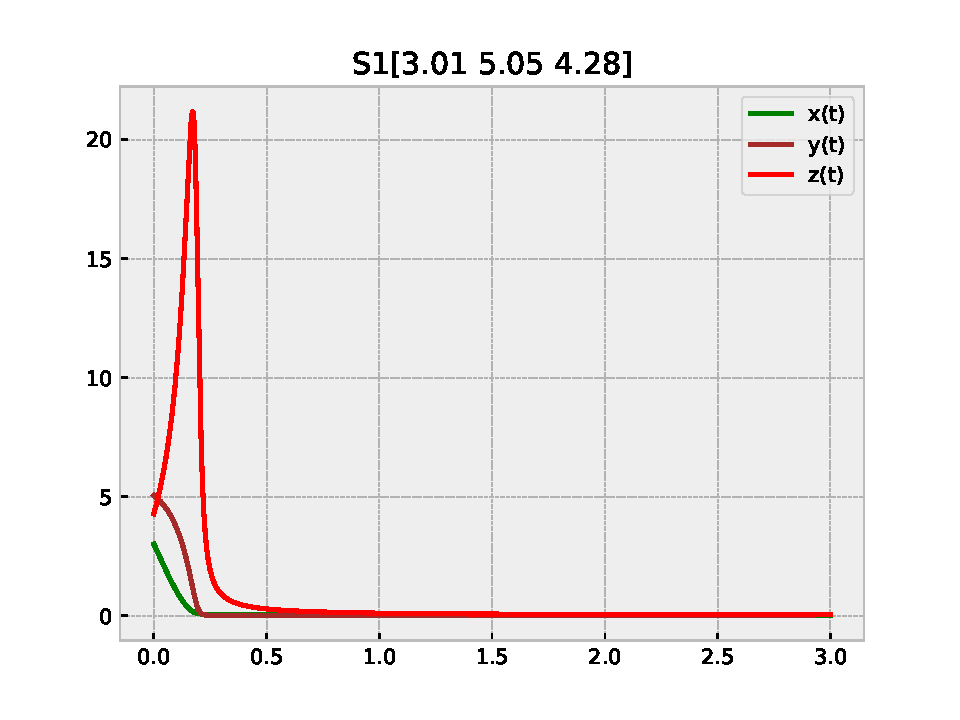
\includegraphics[width=\textwidth]{Simulations/S1[3.01 5.05 4.28].pdf}
				\label{fig:grafica1}
			\end{subfigure}%
			\begin{subfigure}[b]{0.5\textwidth}
				\centering
				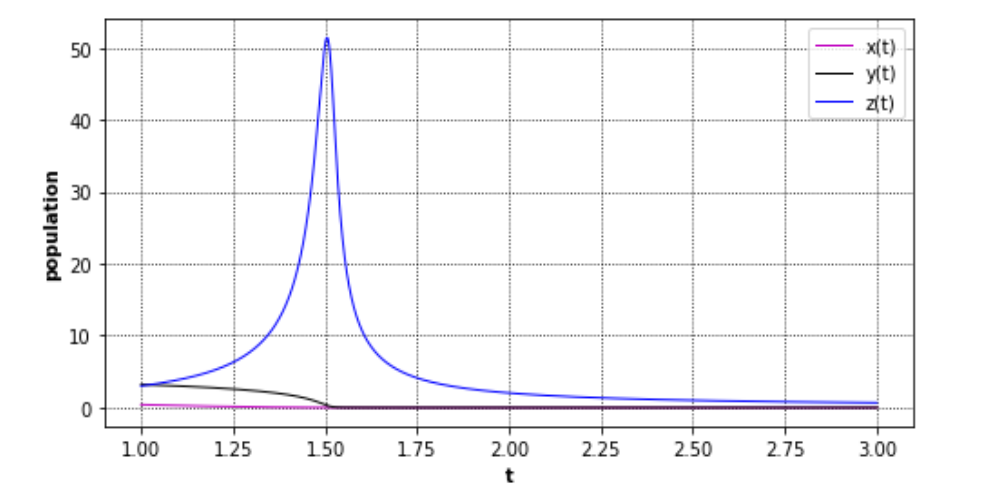
\includegraphics[width=\textwidth]{GraficasPaper/S1[1].png}
				\label{fig:grafica12}
			\end{subfigure}
			\caption{S1 con valores iniciales [3.01 5.05 4.28]}
			\label{fig:comparacion1}
		\end{figure}

	\end{minipage}
\end{frame}


% \begin{frame}
% 	\frametitle{Simulaciones Num\'ericas}
% 	\begin{minipage}{10cm}
% 		\begin{figure}[H]
% 			\centering
% 			\begin{subfigure}[b]{0.5\textwidth}
% 				\centering
% 				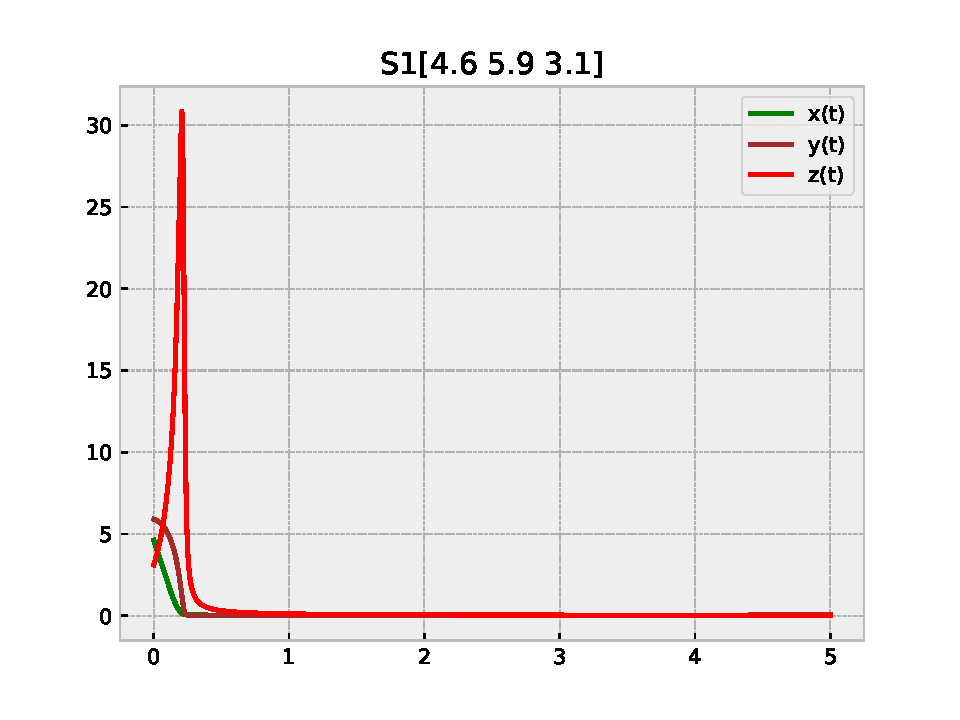
\includegraphics[width=\textwidth]{Simulations/S1[4.6 5.9 3.1].pdf}

% 			\end{subfigure}%
% 			\begin{subfigure}[b]{0.5\textwidth}
% 				\centering
% 				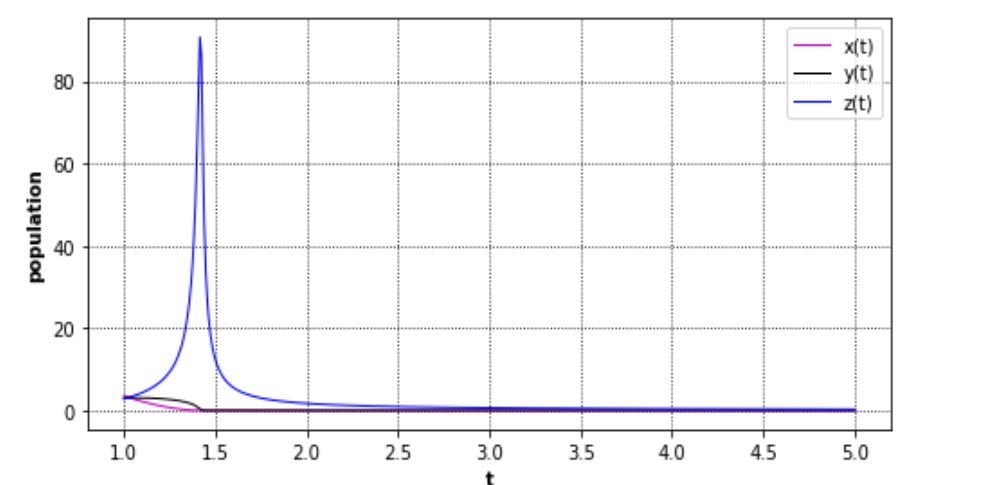
\includegraphics[width=\textwidth]{GraficasPaper/S1[2].png}
% 			\end{subfigure}
% 			\caption{S1 con valores iniciales [4.6 5.9 3.1]}
% 		\end{figure}

% 	\end{minipage}
% \end{frame}

% \begin{frame}
% 	\frametitle{Simulaciones Num\'ericas}
% 	\begin{minipage}{10cm}
% 		\begin{figure}[H]
% 			\centering
% 			\begin{subfigure}[b]{0.5\textwidth}
% 				\centering
% 				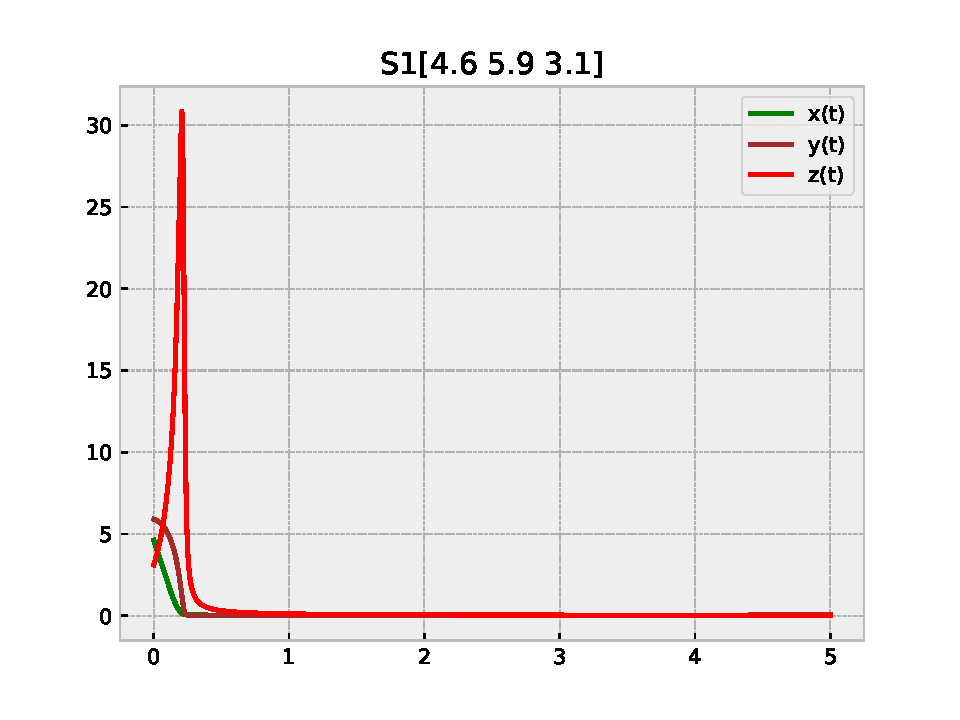
\includegraphics[width=\textwidth]{Simulations/S1[4.6 5.9 3.1].pdf}

% 			\end{subfigure}%
% 			\begin{subfigure}[b]{0.5\textwidth}
% 				\centering
% 				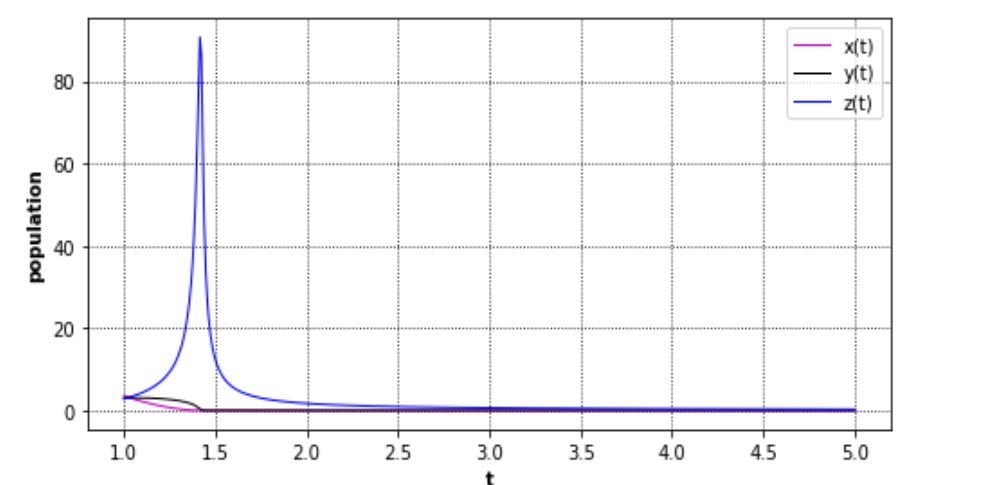
\includegraphics[width=\textwidth]{GraficasPaper/S1[2].png}
% 			\end{subfigure}
% 			\caption{S1 con valores iniciales [4.6 5.9 3.1]}

% 		\end{figure}

% 	\end{minipage}
% \end{frame}


\begin{frame}
	\frametitle{Conclusiones}
	\begin{minipage}{10cm}
		Se ha demostrado para el sistema
	\end{minipage}
\end{frame}

% \begin{frame}
% 	\frametitle{Conclusiones}
% 	\begin{minipage}{10cm}
% 		Se ha demostrado para el sistema
% 	\end{minipage}
% \end{frame}

\begin{frame}
	\frametitle{Recomendaciones}
	\begin{minipage}{10cm}
		Se puede extender los resultados a modelos...
	\end{minipage}
\end{frame}
%----------------------------------
\section{Bibliograf\'ia del tema}
\begin{frame}
	\frametitle{Bibliograf\'ia}
	\begin{thebibliography}{99}

		\bibitem[Sanjuan,2016]{sanjuan2016} M. A. Fern\'andez Sanju\'an (2016). Din\'amica No Lineal, Teor\'ia del Caos y Sistemas Complejos: una perspectiva hist\'orica. {\em Rev. R. Acad. Cienc. Exact. F\'is .Nat.} \textbf{Vol}. 109, N. 1?2, pp. 107-126.
	\end{thebibliography}
\end{frame}

\end{document}

